\documentclass{article}\usepackage[]{graphicx}\usepackage[]{color}
%% maxwidth is the original width if it is less than linewidth
%% otherwise use linewidth (to make sure the graphics do not exceed the margin)
\makeatletter
\def\maxwidth{ %
  \ifdim\Gin@nat@width>\linewidth
    \linewidth
  \else
    \Gin@nat@width
  \fi
}
\makeatother

\definecolor{fgcolor}{rgb}{0.345, 0.345, 0.345}
\newcommand{\hlnum}[1]{\textcolor[rgb]{0.686,0.059,0.569}{#1}}%
\newcommand{\hlstr}[1]{\textcolor[rgb]{0.192,0.494,0.8}{#1}}%
\newcommand{\hlcom}[1]{\textcolor[rgb]{0.678,0.584,0.686}{\textit{#1}}}%
\newcommand{\hlopt}[1]{\textcolor[rgb]{0,0,0}{#1}}%
\newcommand{\hlstd}[1]{\textcolor[rgb]{0.345,0.345,0.345}{#1}}%
\newcommand{\hlkwa}[1]{\textcolor[rgb]{0.161,0.373,0.58}{\textbf{#1}}}%
\newcommand{\hlkwb}[1]{\textcolor[rgb]{0.69,0.353,0.396}{#1}}%
\newcommand{\hlkwc}[1]{\textcolor[rgb]{0.333,0.667,0.333}{#1}}%
\newcommand{\hlkwd}[1]{\textcolor[rgb]{0.737,0.353,0.396}{\textbf{#1}}}%
\let\hlipl\hlkwb

\usepackage{framed}
\makeatletter
\newenvironment{kframe}{%
 \def\at@end@of@kframe{}%
 \ifinner\ifhmode%
  \def\at@end@of@kframe{\end{minipage}}%
  \begin{minipage}{\columnwidth}%
 \fi\fi%
 \def\FrameCommand##1{\hskip\@totalleftmargin \hskip-\fboxsep
 \colorbox{shadecolor}{##1}\hskip-\fboxsep
     % There is no \\@totalrightmargin, so:
     \hskip-\linewidth \hskip-\@totalleftmargin \hskip\columnwidth}%
 \MakeFramed {\advance\hsize-\width
   \@totalleftmargin\z@ \linewidth\hsize
   \@setminipage}}%
 {\par\unskip\endMakeFramed%
 \at@end@of@kframe}
\makeatother

\definecolor{shadecolor}{rgb}{.97, .97, .97}
\definecolor{messagecolor}{rgb}{0, 0, 0}
\definecolor{warningcolor}{rgb}{1, 0, 1}
\definecolor{errorcolor}{rgb}{1, 0, 0}
\newenvironment{knitrout}{}{} % an empty environment to be redefined in TeX

\usepackage{alltt}

\title{Comparing Mechanistic and Statistical Models to Forecast Influenza in the U.S.}

\author{Logan Brooks, Spencer Fox, Craig McGowan, Sasikiran Kandula, \\ Dave Osthus, Evan Ray, Nicholas G Reich, Roni Rosenfeld, Jeffrey Shaman, \\Abhinav Tushar, Teresa Yamana [authorship list to be finalized]}

\usepackage[letterpaper, margin=1in]{geometry} % margin
\usepackage{lineno}% add line numbers
\usepackage{graphicx}
\usepackage[colorlinks=true, allcolors=blue]{hyperref}
\usepackage{parskip}        % for spacing after paragraphs http://ctan.org/pkg/parskip
\usepackage{url}            % simple URL typesetting
\usepackage{booktabs}       % professional-quality tables
\usepackage{amsfonts}       % blackboard math symbols
\usepackage{nicefrac}       % compact symbols for 1/2, etc.
\usepackage{amsmath, amsfonts}
\usepackage{setspace}
\linenumbers % line numbers
\onehalfspacing



% For computer modern sans serif
\usepackage[T1]{fontenc}
\renewcommand*\familydefault{\sfdefault} %% Only if the base font of the document is to be sans serif
\IfFileExists{upquote.sty}{\usepackage{upquote}}{}
\begin{document}

\maketitle

\tableofcontents




\section{Introduction}
Forecasts of infectious disease outbreaks can inform public health response to outbreaks. Close collaboration between public health policy-makers and quantitative modelers is necessary to ensure the forecasts have maximum impact and are appropriately communicated to the public and the broader public health community. 

Infectious disease modeling has proven to be fertile ground for statisticians, mathematicians, and quantitative modelers for over a century. Yet there is not a consensus on a single best modeling approach or method for forecasting the dynamic patterns of infectious disease outbreaks, in both endemic and emergent settings. Mechanistic models consider the biological underpinnings of disease transmission, and are in practice are typically implemented as variations on the Susceptible-Infectious-Recovered (SIR) model. Phenomenological models largely ignore the biological underpinnings and theory of disease transmission and focus instead on using data-driven, empirical and statistical approahces to make the best forecasts possible of a given dataset, or phenomenon. Both approaches are commonly used and both have advantages and disadvantages in different settings.   


\section{Methods}

\subsection{FluSight Challenge Overview}

Starting in the 2013-2014 influenza season, the CDC has run the "Forecast the Influenza Season Collaborative Challenge" (a.k.a. FluSight) each influenza season, soliciting weekly forecasts for specific influenza season metrics from teams across the world. These forecasts are displayed together on a website during the season and are evaluated for accuracy after the season is over.\cite{PhiResearchLab} 
Detailed methodology and results from this challenge have been published\cite{Biggerstaff2016}, but summarize the key features of the challenge here.

The FluSight challenge has been focused on forecasts of the weighted percentage of doctor's office visits for influenza-like-illness (wILI) in a particular region. This is a standard measure of seasonal flu activity, for which public data is available back to the 1997/1998 influenza season. During each influenza season, this data is updated each week by the CDC (Figure \ref{fig:timezero-schematic}). When the most recent data is released, the prior weeks' reported wILI data may also be revised. The unrevised data, available at a particular moment in time, is available via the DELPHI real-time epidemiological data API beginning in the 2013/2014 season.\cite{DELPHI} This API enables researchers to ``turn back the clock'' to a particular moment in time and use the data available at that time. This enables more accurate assessment of how models would have performed in real-time. 

\begin{figure}[htbp]
\begin{center}
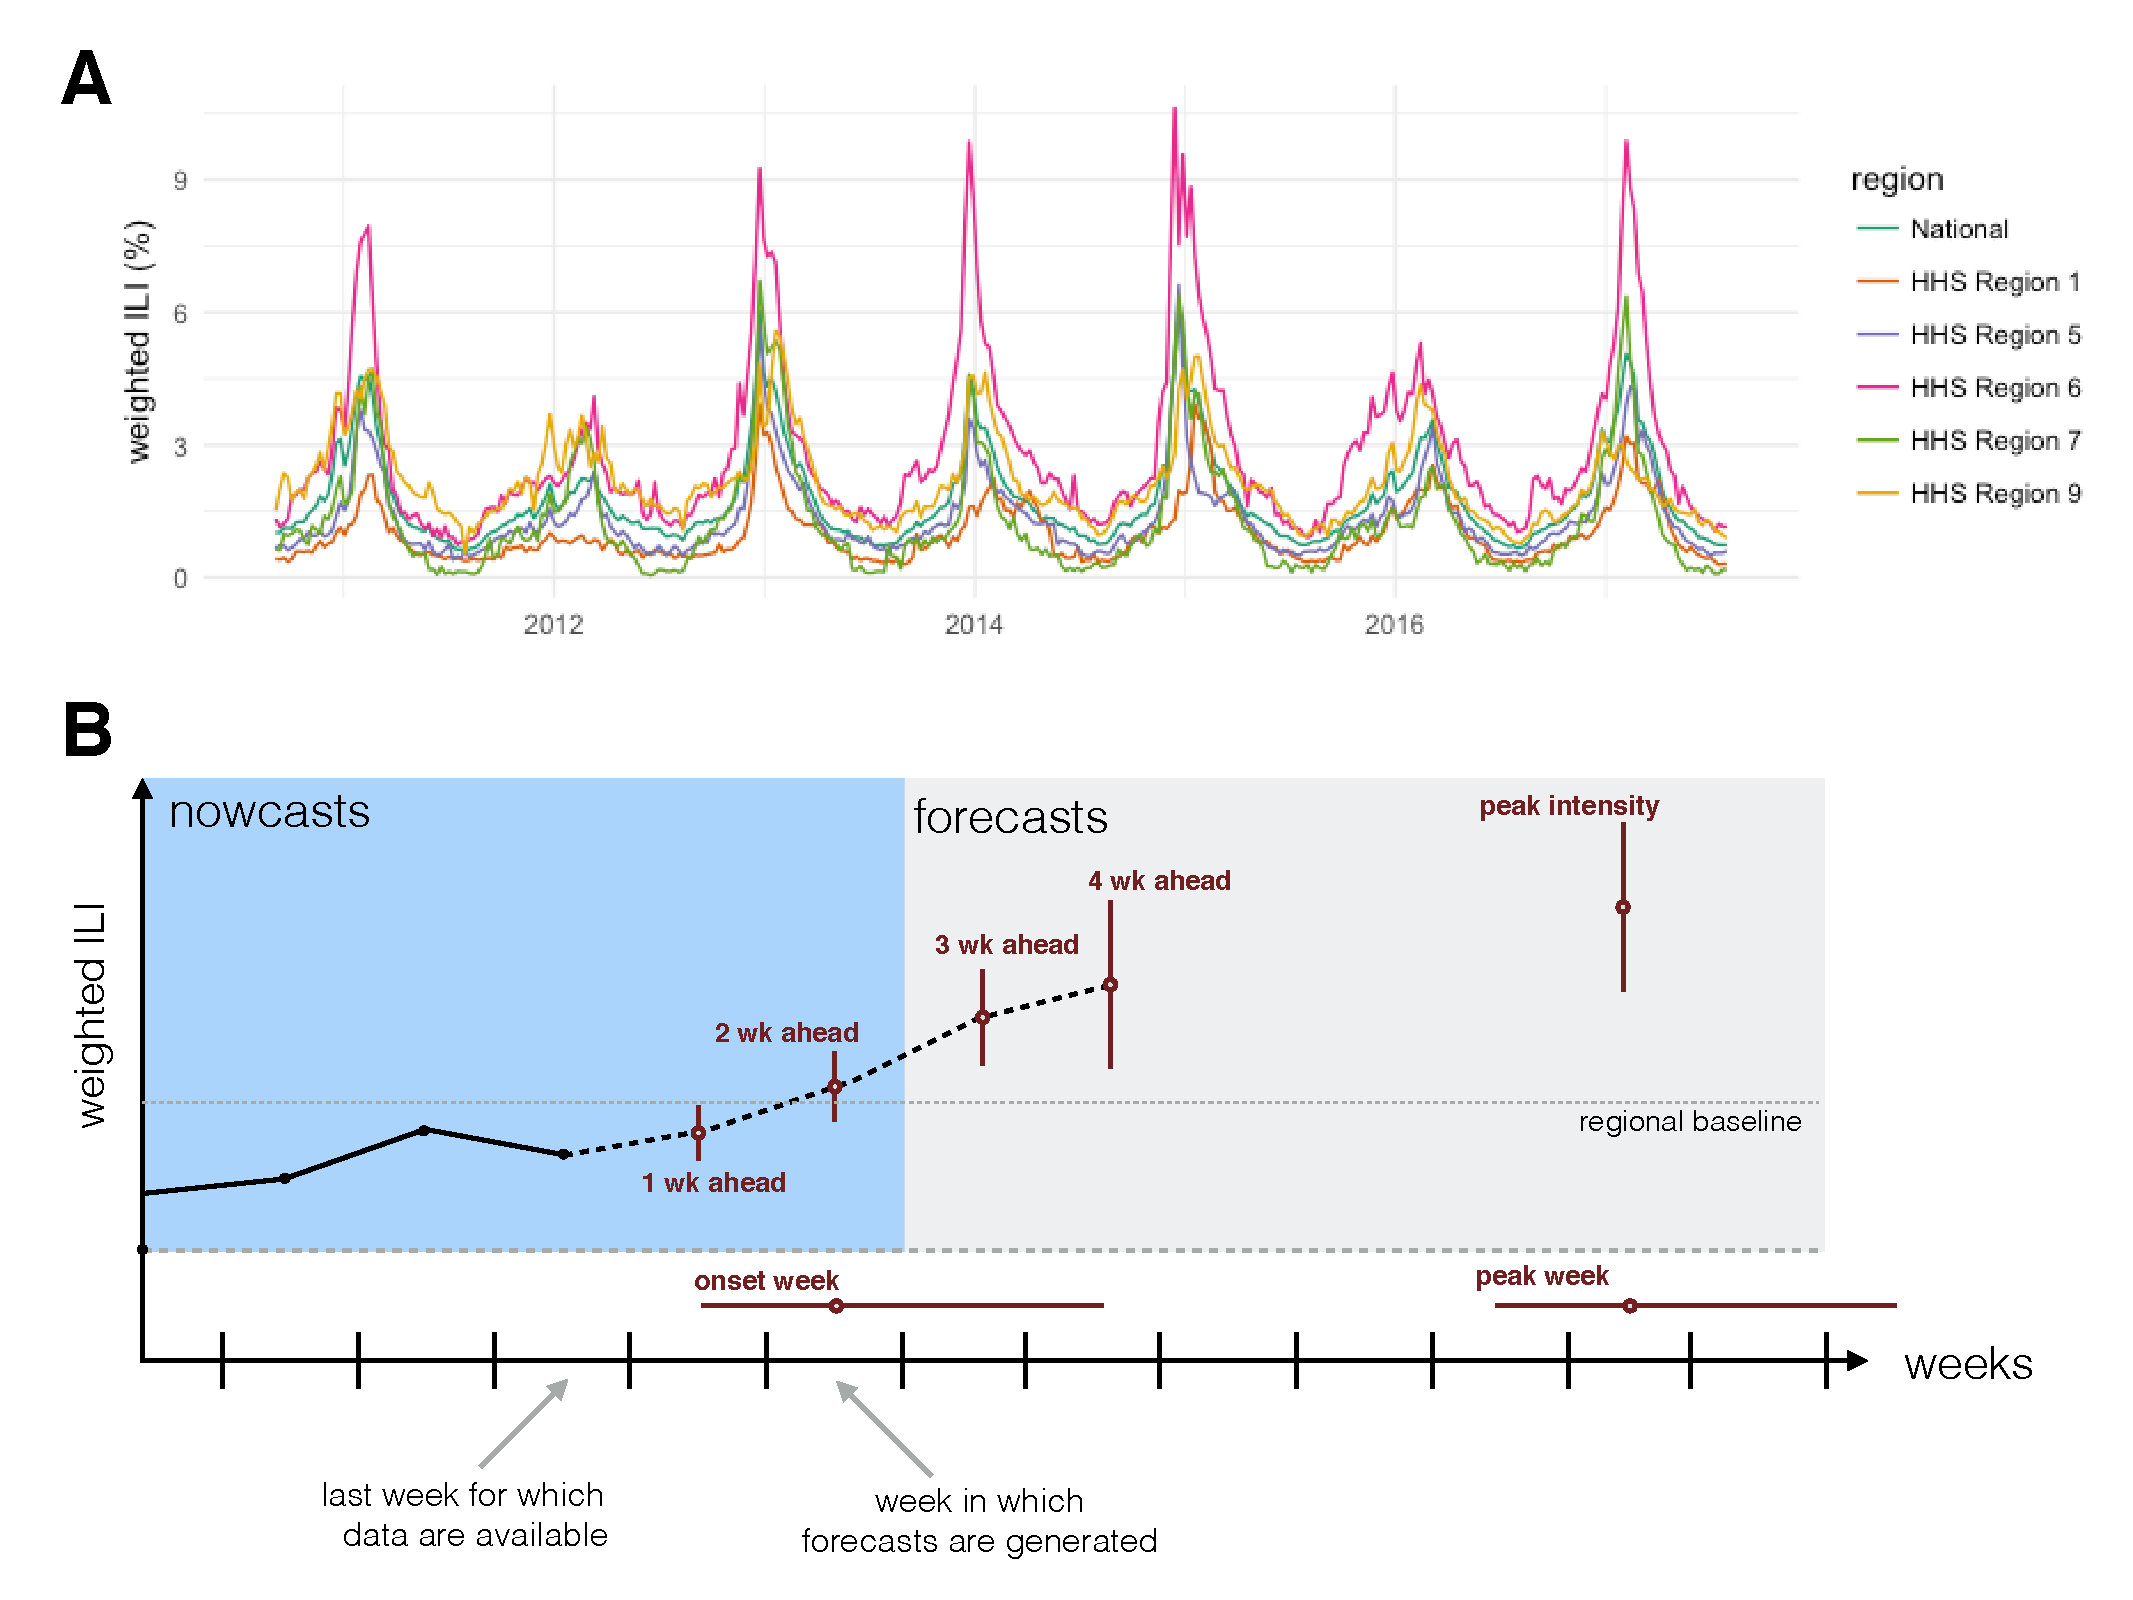
\includegraphics[width=\textwidth]{static-figures/timezero-sketch.pdf}
\caption{A schematic showing when data arrives in realtime relative to when the forecasts are made available.}
\label{fig:timezero-schematic}
\end{center}
\end{figure}


The FluSight challenges have defined seven forecasting targets of particular public health relevance. Three of these targets are fixed scalar values for a particular season: onset week, peak week, and peak intensity (i.e. the maximum observed wILI percentage). The remaining four targets are the observed wILI percentages in each of the subsequent four weeks. 

The FluSight challenges have also required that all forecast submissions and follow a particular format. A single submission file (a comma-separated text file) contains the forecast made for a particular epidemic week (EW) of a season. Standard CDC definitions of epidemic week are used. Each file contains binned predictive distributions for seven specific targets across the 10 HHS regions of the US plus the national level. Each file contains over 8000 rows and typically is about 400KB in size.

To be included in the model comparison presented here, previous participants in the CDC FluSight challenge were invited to provide out-of-sample forecasts for the 2010/2011 through 2016/2017 seasons. For each model, this involved creating 233 separate forecast submission files, one for each of the weeks in the seven training seasons.
Each forecast file represented a single submission file, as would be submitted to the CDC challenge. 
Each team created their submitted forecasts in a prospective, out-of-sample fashion, i.e. fitting or training the model only on data available before the time of the forecast (see Figure \ref{fig:timezero-schematic}). 

\subsection{Description of this Forecasting Experiment}


\subsection{Summary of Models}

Particular reference to the 2-3 models that can be considered ``baseline'' models:
 - Delphi-Uniform
 - ReichLab-KDE

see Table \ref{tab:model-list}

%% Table with columns for:
%%   - institution
%%   - model name
%%   - underlying method
%%   - statistical/mechanistic
%%   - non-ILI data sources

\begin{table}
\setlength{\tabcolsep}{4pt} 
\begin{tabular}{p{1.6cm} l p{7.5cm} l  p{1cm}  p{1cm} p{1cm}}
\hline
Team     & Model Abbr& Model Description & & Ext. Data & Mech. Model & Ens. Model \\ 
\hline
CU       & EAKFC\_SEIRS       & Ensemble Adjustment Kalman Filter SEIRS & \cite{Pei2018}  & x & x & \\ 

~        & EAKFC\_SIRS        & Ensemble Adjustment Kalman Filter SIRS & \cite{Pei2018}  & x & x & \\
~        & EKF\_SEIRS         & Ensemble Kalman Filter SEIRS & \cite{Yang2017}    & x             & x &                    \\
~        & EKF\_SIRS          & Ensemble Kalman Filter SIRS & \cite{Yang2017}     & x             & x   &                 \\
~        & RHF\_SEIRS         & Rank Histogram Filter SEIRS & \cite{Yang2017}    & x             & x     &               \\
~        & RHF\_SIRS          & Rank Histogram Filter SIRS & \cite{Yang2017}     & x             & x       &             \\
~        & BMA                & Bayesian Model Averaging & \cite{Yamana2017}      & ~             & ~          &          \\
\hline
Delphi   & BasisRegression    & Basis Regression ({\tt epiforecast} defaults) & \cite{Brooks2015a} & ~             & ~     &               \\ 
~        & DeltaDensity1      & Delta Density ({\tt epiforecast} defaults)   & \cite{Brooks2015a} & ~             & ~       &             \\ 
~        & EmpiricalBayes1    & Empirical Bayes (conditioning on past four weeks) & \cite{Brooks2015,Brooks2015a} & ~             & ~  &                  \\ 
~        & EmpiricalBayes2    & Empirical Bayes ({\tt epiforecast} defaults) & \cite{Brooks2015,Brooks2015a} & ~             & ~            &        \\ 
~        & EmpiricalFuture    & Empirical Futures ({\tt epiforecast} defaults) &  \cite{Brooks2015a} & ~             & ~         &           \\ 
~        & EmpiricalTraj      & Empirical Trajectories ({\tt epiforecast} defaults)& \cite{Brooks2015a} & ~             & ~         &           \\ 
~        & DeltaDensity2      & Markovian Delta Density ({\tt epiforecast} defaults)& \cite{Brooks2015a} & ~             & ~          &          \\ 
~        & Uniform            & Uniform Distribution&  & ~             & ~   &                 \\ 
~        & Stat               & Ensemble (combination of 8 Delphi models)& & ~             & ~  & x                 \\
\hline
LANL     & DBM                & Dynamic Bayesian SIR Model with discrepancy & \cite{Osthus2017} & ~             & x      &              \\ 
\hline
ReichLab & KCDE               & Kernel Conditional Density Estimation & \cite{Ray2017}  & ~             & ~            &        \\ 
~        & KDE                & Kernel Density Estimation and penalized splines & \cite{Ray2018}  & ~             & ~     &               \\ 
~        & SARIMA1            & SARIMA model without seasonal differencing & \cite{Ray2018} & ~             & ~      &              \\ 
~        & SARIMA2            & SARIMA model with seasonal differencing & \cite{Ray2018} & ~             & ~           &         \\ 
\hline
UTAustin & EDM                & Empirical Dynamic Model, or method of analogues & \cite{Sugihara1990} & ~             & ~         &           \\ 
\end{tabular}
\caption{List of models, with key characteristics. Team abbreviations are translated as: CU = Columbia University, Delphi = Carnegie Mellon, LANL = Los Alamos National Laboratories, ReichLab = University of Massachusetts Amherst, UTAustin = University of Texas Austin.  The `Ext data' column notes models that use data external to the ILINet data from CDC. The `Mech. model' column notes models that rely to some extent on an mechanistic or compartmental model formulation. The `Ens. model' column notes models that are ensemble models.}
\label{tab:model-list}
\end{table}

\subsection{Metrics Used for Evaluation and Comparison}

Forecasts have historically been evaluated by the CDC using two metrics, the log-score and the mean absolute error. These two metrics capture different desirable features of performance. The log-score enables evaluation of both the precision and accuracy of a forecast, using the predicted density function.\cite{Gneiting2007} The absolute error provides an interpretable summary of the amount of error the point estimates had on average.\cite{Reich2016} 

We used a modified form of the log-score to evaluate forecasts, in line with the evaluation performed by the CDC. The log-score is defined as $\log f(\hat z|\bf{x})$ where $f(z|\bf{x})$ is a predictive density function for some target $z$, conditional on some data $\bf{x}$ and $\hat z$ is the observed value of the target $z$. In practice, each model $m$ has a set of log scores associated with it are region-, target-, season-, and week- specific, notated as $\log f^{(m)}_{r,t,s,w}(\hat z|\bf{x})$. We evaluated model performance based on the exponentiated average log scores, which has been called ``forecast skill'' and is equivalent to the geometric mean of the probabilities assigned to the eventually observed outcome. 
For example, the forecast skill for model $m$ and target $t$ would be calculated as
\begin{eqnarray}
 FS^{m}_{t} & = & \exp \left ( \frac{1}{N} \sum_{r,s,w} \log \hat f^{(m)}_{r,t,s,w}(\hat z|{\bf x}) \right ) \\
 & = & \left ( \prod_{r,s,w} \hat f^{(m)}_{r,s,w}(\hat z|{\bf x}) \right ) ^{1/N} 
\end{eqnarray}
where $N$ is the total number of log-scores for target $t$ and model $m$, across all combinations of region, season, and week. 
Further, within a given region-season-target combination, the weeks included in the calculation of the average forecast skill depend on when the onset and peak occur. Specifically, [[...]].
All weeks are included for the forecast skill calculations for the $k$-step ahead forecasts of wILI.

The log-scores are computed for the targets on the wILI percentage scale such that predictions within +/- 0.5 percentage points are considered accurate, i.e. log score = $\log \int_{\hat z -.5}^{\hat z + .5} f^{(m)}(z|{\bf{x}})dz$. For the targets on the scale of epidemic weeks, predictions within +/- 1 week are considered accurate, i.e. log score = $\log \int_{\hat z -1}^{\hat z + 1} f^{(m)}(z|{\bf{x}})dz$. 
\begin{itemize}
    \item log-score for predictive distribution, aggregated by (model), (model x season), (model x season x location), (model x season x target-type), (model x season x target), , (model x season x week)
    \item MAE for point predictions
\end{itemize}

\subsection{Formal comparisons of model performance}

\begin{itemize}
    \item permutation test for pairwise statistical comparison between two models
    \item beta regression or permutation test for comparison between groups of models (i.e. mechanistic vs. statistical)
\end{itemize}


\section{Results}

Things to confirm: removed weeks that CDC does not score, no onset seasons and multi peak years are handled appropriately

\subsection{Performance in forecasting week-ahead incidence}

Average forecast skill for the four week-ahead targets varied substantially across models and regions.
The best model (XX) achieved between XX and XX average skill in forecasting week-ahead targets across all seasons and regions.
The historical baseline model achieved between XX and XX average skill.
Of the XX model-region-seasons available for comparison to the historical baseline, XX\% showed greater skill than the historical baseline for a given region-season.


Even within given models, forecast skill showed large region-to-region and year-to-year variation. 
The model with the lowest variation in forecast skill across region-seasons was XX, with skills ranging between XX and XX.
The model with the highest variation in forecast skill across region-seasons was XX, with skills ranging between XX and XX.
In general, Region XX was the easiest to forecast and XX was the hardest, with models showing an average forecast skill of XX and XX across all seasons, respectively.

Forecast skill declined as the target moved further into the future.
For the model with highest forecast skill across all four week-ahead targets (XX), the average skill across region and season for 1 through 4 week-ahead forecasts were XX, XX, XX and XX.
This mirrored an overall decline in skill observed across most models.
The historical baseline model showed average forecast skill of XX for all week-ahead targets. (Performance does not decline for the historical model, since it always forecasts the same thing for every week, without updating based on recent data.)
For 1 week-ahead forecasts, XX of 21 models showed more skill than a historical baseline. 
For the 4 week-ahead forecasts, only XX of 21 models showed more skill than the historical baseline.
In Regions XX, XX, and XX, the average forecast skill for the ``nowcast'' targets (1 and 2 weeks ahead) were both above 0.5.


\subsection{Performance in forecasting seasonal targets}

Of the three seasonal targets, models showed the lowest average skill in forecasting season onset, with an overall average skill of XX. 
Due to the variable timing of season onset, different numbers of weeks were included in the final scoring for each region-season, varying from XX to XX weeks per region-season (see methods for details).
Of the XX region-seasons evaluated, XX had no onset. 
The best model for onset was XX, with overall average skill of XX and minimum skill for a region-season of XX.
Overall, XX of XX models had more forecast skill than the historical baseline model in the scoring period of interest.


Models showed less overall skill in forecasting the peak week and peak intensity when compared to the week-ahead forecasts.
Model-specific average skill for peak week, across region and season, was above 0.25 for XX models. 
This means that XX models assigned on average at least 25\% probability to a week within +/- 1 week of the eventually observed peak week during the scoring period of interest.
Similarly, for peak intensity, XX models assigned on average at least 25\% probability to a wILI percentage within +/- 0.5\% of the eventually observed value during the scoring period of interest.
During the same time-periods, the historical model forecasts assigned XX\% probability to the eventually observed peak week and XX\% probability to the eventually observed peak intensity.

Average forecast skill showed substantial variation by region and by season.
[[Forecasts of peak intensity and peak week showed lower skill in seasons that experienced higher than average peak incidence.]]
[[Forecasts of peak intensity and peak week showed lower skill in regions with larger variability in peak incidence.]]

\subsection{Characterize skill and variability in skill of each model}

TODO: make point plot of skill by season to show variability and average performance.

\begin{figure}[htbp]
\begin{center}
\includegraphics[width=\textwidth]{figures/fig-results-model-season.pdf}
\caption{Model forecast season, overall and by season. Models are sorted from least skill (left) to most skill (right). Dots show average skill across all targets and regions for a given season. The x marks the average of the seven seasons. The names of compartmental models are shown in bold face. The ReichLab-KDE model can be thought of as the historical baseline model.}
\label{fig:results-season}
\end{center}
\end{figure}



\subsection{Performance of models by location}

Consider adding map that averages across all models, or shows max skill per region, as it varies quite a bit.

\begin{figure}[htbp]
\begin{center}
\includegraphics[width=\textwidth]{figures/fig-results-region.pdf}
\caption{Model results by region and target-type.}
\label{fig:results-region}
\end{center}
\end{figure}


two columns: by target type
mapa: average performance across all models(-KDE)/targets by region
mapb: performance of historical model by region
figc: scatter plot of region-level historical model skill on x and avg model skill on y, colored by season


\subsection{Comparison between statistical and compartmental models}


Statistical models showed the same amount of skill as compartmental models at forecasting week-ahead targets, and slightly more skill for the seasonal targets. 
Using the best three overall models from each category, we computed the average forecast skill for each combination of region, season, and target (Table \ref{tab:score-by-model-type}). 
For the week-ahead forecasts, the difference in model skill was below XX.
For the three seasonal targets, the difference in model skill was larger, ranging from XX for [target X] to XX for [target X].
We note that the 1 week-ahead forecasts from the compartmental models from the CU team are driven largely by a statistical ``nowcast`` model that uses data from the Google Search API and influenza laboratory testing data from the CDC to create the ILI+ metric.\cite{yang2014}
Therefore, the only truly compartmental model making 1 week-ahead forecasts is the LANL-DBM model. 

% latex table generated in R 3.5.1 by xtable 1.8-3 package
% Tue Dec  4 20:17:56 2018
\begin{table}[ht]
\centering
\begin{tabular}{lrrr}
   \hline 
 & \multicolumn{2}{c}{score} &  \\
target & stat. model & comp. model & diff. \\ 
  \hline
1 wk ahead & 0.49 & 0.43 & 0.06 \\ 
  2 wk ahead & 0.40 & 0.41 & -0.01 \\ 
  3 wk ahead & 0.35 & 0.34 & 0.00 \\ 
  4 wk ahead & 0.32 & 0.30 & 0.02 \\ 
  Season onset & 0.23 & 0.22 & 0.01 \\ 
  Season peak percentage & 0.32 & 0.27 & 0.05 \\ 
  Season peak week & 0.34 & 0.32 & 0.02 \\ 
   \hline
\end{tabular}
\caption{Comparison of the top three statistical models ({\tt Delphi-DeltaDensity1}, {\tt ReichLab-KCDE}, {\tt ReichLab-SARIMA2}) and the top three compartmental models, ({\tt LANL-DBM}, {\tt CU-EKF\_SIRS}, {\tt CU-RHF\_SIRS}) based on best average region-season forecast score. The diff. column represents the difference in the average probability assigned to the eventual outcome for the target in each row. Positive values indicate the top statistical models showed higher average score than the top compartmental models.} 
\label{tab:score-by-model-type}
\end{table}



% Gamma mixed effects regression model on negative log-scores. Need to remove correlation between successive observation.
% 
% strategies to remove correlation between successive scores within a year:
% \begin{itemize}
%     \item smooth/aggregate scores into different sections of the year, possibly reducing the number of and/or correlation between sucessive scores
%     \item smooth spline across years with random effect for model, fixed effects for model-type
%     \item permutation test
% \end{itemize}


\subsection{Where do these models fail?}

\begin{itemize}
    \item holiday peak?
    \item data revisions
    \item peak performance? (connection between size of season and performance)
    \item missing a slow descent because of a second outbreak that is lifting the tail up?
\end{itemize}


\section{Discussion}

\subsection{Overview of key results and importance}
The first large-scale comparison of flu forecasting models from different modeling teams/philosophies across multiple years.

\subsection{Overview of statistical vs. mechanistic model comparison}
As our knowledge/data about the system mature, we expect mechanistic models to be better, but when true signals of mechanistic model is drowned out by observational noise or spatial aggregation, statistical models may perform better. This comparison serves as a barometer for where the current state of forecast models are.

\subsection{Limitations}

\begin{itemize}
    \item relatively few additional data sources incorporated
    \item no models that explicitly incorporate strain information
    \item no models with spatial information included
    \item seven seasons of data is not a lot (n=7) to draw strong conclusions about comparative model performance
    \item currently limited to models with only recent data...
\end{itemize}

\bibliographystyle{unsrt}
\bibliography{../flusightnetwork.bib}

\end{document}
